\documentclass[a4paper, 11pt]{scrartcl}

\usepackage[utf8]{inputenc}
\usepackage[T1]{fontenc}
\usepackage[ngerman]{babel}

\usepackage{amssymb}
\usepackage{amsmath}

\usepackage{float}
\usepackage{listings}
\usepackage{framed}
\usepackage{caption}
\usepackage{url}

\usepackage{chessboard}
\usepackage{color}

\lstset{language=C, basicstyle=\footnotesize\ttfamily}

\setlength\parindent{0pt}

\title{36.\ Bundeswettbewerb Informatik\\Aufgabe 5\\Bauernopfer\\Dokumentation}
\author{Kamal Abdellatif}
\date{\today}

\storechessboardstyle{static}{showmover=false}
\storechessboardstyle{table}{
	showmover=false, marginwidth=8pt, printarea=e1-h3, hlabel=false, pgfstyle=straightmove, arrow=to
}

\begin{document}
\maketitle

\section*{Treibjagd}
Ziel der Bauern ist es, die Zugmöglichkeiten des Turms einzugrenzen. Steht dem Turm viel freie Fläche zur Verfügung, so kann er nur schwer gefangen werden, da viele Ausweichmöglichkeiten vorhanden sind. Wird der Turm jedoch nach und nach in seinen Möglichkeiten eingegrenzt, so kann er schließlich immer gefangen werden. Die folgend beschriebene Strategie versucht, die Möglichkeiten des Turms ausgänglich von einer gegebenen Anfangsstellung zu minimieren. Damit das Programm mögliche Vorstöße der Bauern bewerten kann, wird eine quantitative Definition der Zugmöglichkeiten des Turms benötigt.

\begin{framed}
	Die \emph{Zugmöglichkeiten} des Turms einer gegebenen Stellung sind die Menge aller Felder, die der Turm in einer endlichen Anzahl von erlaubten Zügen ausgehend von seiner aktuellen Position erreichen kann.
\end{framed}
Erlaubte Züge des Turms sind alle Züge, die horizontal oder vertikal von einer Startposition zu einer Endposition verlaufen, ohne dabei einen Bauern zu überspringen. Die Endposition darf dabei kein Feld sein, welches von einem Bauern besetzt oder bedroht ist. Ein \emph{bedrohtes Feld} ist ein Feld, das in einem Zug von einem Bauern erreicht werden kann. Der Turm gilt als gefangen, wenn er keine Zugmöglichkeiten mehr besitzt.
\newpage
Würde der Turm auf ein solches Feld ziehen, so würde er sofort geschlagen werden können. Es kann davon ausgegangen werden, dass der Turm optimal spielt. Daher wird der Turm nie ein bedrohtes Feld besuchen.

Die möglichen erreichbaren Felder sind rekursiv definiert:\\\\
\textsc{Rekursionsanfang}\\ Die aktuelle Position des Turms ist erreichbar. \\\\
\textsc{Rekursionsschritt}\\ Ist ein Feld erreichbar, so sind es alle Felder, auf die der Turm von diesem Feld aus ziehen könnte, auch.

\begin{minipage}[t]{.5\textwidth}
	\centering
	\chessboard[style=static,
		setpieces={Pa3, Ph2, Pc4, Pf4, Pg5, Pe6, Pc7, Pd8},
		markstyle=color,
		pgfcolor=red,
		pgfopacity=.25,
		markfields={
			a2, b3, a4, c3, c5, b4, d4, h1, h3, g2, f3, f5, e4, h5, g6, d6, f6, e7, b7, d7, c8, e8, a3, h2, c4, f4, g5, e6, c7, d8, c6, g4, e5
		}
	]
	\captionof{figure}{Bedrohte Felder (rot)}
\end{minipage}
\hfill
\begin{minipage}[t]{.5\textwidth}
	\centering
	\chessboard[style=static,
		setpieces={ra1, Pa3, Ph2, Pc4, Pf4, Pg5, Pe6, Pc7, Pd8},
		markstyle=color,
		pgfcolor=red,
		pgfopacity=.25,
		markfields={
			a2, b3, a4, c3, c5, b4, d4, h1, h3, g2, f3, f5, e4, h5, g6, d6, f6, e7, b7, d7, c8, e8, a3, h2, c4, f4, g5, e6, c7, d8, c6, g4, e5
		},
		markstyle=color,
		pgfcolor=blue,
		markfields={d5, g3, b8},
		markareas={a1-g1, b2-f2, d3-e3, a5-a8, b5-b6}
	]
	\captionof{figure}{Erreichbare Felder (blau)}
	\label{fig:erreib}
\end{minipage}

\vspace*{1em}
Die Bauern folgen einer Einschnürungs-Strategie. Dabei sollen die Zugmöglichkeiten stetig verringert werden. Demzufolge ist ein Bauernzug, der die Anzahl von erreichbaren Feldern vergrößert, nicht Teil der Strategie. Ein solcher Zug wird als \emph{Öffnung} bezeichnet. So kann ein Zug auf den ersten Blick harmlos erscheinen, dem Turm aber ein Schlupfloch verschaffen. Ein Beispiel dafür wäre hier der Zug e6$\rightarrow$e5. Solange keine Öffnung auftritt, gilt die Bauernstellung als \emph{geschlossen}.
\begin{figure}[H]
	\centering
	\chessboard[style=static,
		setpieces={ra1, Pa3, Ph2, Pc4, Pf4, Pg5, Pe6, Pc7, Pd8},
		pgfstyle=straightmove,
		arrow=to,
		markmoves={e6-e5},
	]
	\chessboard[style=static,
		setpieces={ra1, Pa3, Ph2, Pc4, Pf4, Pg5, Pe5, Pc7, Pd8},
		pgfstyle=straightmove,
		pgfcolor=blue,
		arrow=to,
		markmoves={a1-d1, d1-d6, d6-f6},
		markstyle=color,
		pgfcolor=red,
		pgfopacity=.25,
		markfields={
			a2, b3, a4, c3, c5, b4, d4, h1, h3, g2, f3, f5, e4, h5, g6, b7, d7, c8, e8, a3, h2, c4, f4, g5, e6, c7, d8, c6, g4, e5, d5
		},
		markstyle=color,
		pgfcolor=blue,
		markfields={g3, b8, d6, f6, h6, h4},
		markareas={a1-g1, b2-f2, d3-e3, a5-a8, b5-b6, e7-h7, f8-h8},
	]
	\caption{Öffnung der Bauernstellung}
\end{figure}
Die Anfangsstellung wurde so gewählt, dass von Anfang an die Möglichkeiten des Turms stark reduziert sind. Wenn die Bauern eine geschlossene Stellung halten, so müssen sie am Anfang das Brett zweiteilen. Da der Turm nach Aufstellung der Bauern sich in das Feld setzen kann, hat der die Möglichkeit, den größeren und somit günstigeren Teil für sich zu wählen. Um diese Wahl so ungünstig wie möglich zu machen, werden beide Hälften gleichgroß gewählt, da der Turm so keinen Vorteil durch die Wahl der Hälfte erhält. Unter diesen Gesichtspunkten wurde folgende Startposition gewählt
\begin{minipage}[t]{.5\textwidth}
	\centering
	\chessboard[style=static, setpieces={Pa3, Pb6, Pc3, Pd6, Pe3, Pf6, Pg3, Ph6}]
	\captionof{figure}{Startposition}
\end{minipage}
\begin{minipage}[t]{.5\textwidth}
	\chessboard[style=static,
		setpieces={Pa3, Pb5, Pc2, Pd5, Pe3, Pf5, Pg3, Ph5},
		markstyle=color,
		pgfcolor=blue,
		pgfopacity=.25,
		markareas={a1-b1, d1-h1},
		markfields={f2, h2}
	]
	\captionof{figure}{Bauernstellung nach 5 Zügen}
\end{minipage}
\newpage
Das Programm beginnt darauf hin, nach jedem Zug des Turms jeden möglichen Bauernzug zu betrachten. Es wählt dabei den Bauernzug, welcher die erreichbaren Felder des Turms am meisten verringert. Obwohl dieses "`greedy"'-Vorgehen kurzsichtig erscheinen mag, ist es dennoch sehr effizient. Mit dem ersten Zug wählt der Turm eine Seite. Auf Grund der Symmetrie wird im Folgenden ohne Beschränkung der Allgemeinheit die untere gewählt. Die ersten 5 Züge der Bauern waren unabhängig vom Verhalten des Turms. Die Bauern auf der 6. Reihe rücken zuerst vor, da diese jeweils mit einem Zug nach vorne ein erreichbares Feld des Turms eleminieren. Dies trifft nicht auf die vorderen Bauern zu, da diese neue Felder hinter sich öffnen würden. Diese Öffnungen sind im 5. Zug abgedeckt, da nun die 5. Reihe besetzt ist. Die Mittelbauern können durch vorrücken 4 Felder eleminieren, die Randbauern nur 3. Demnach zieht immer zuerst einer der Mittelbauern.

Je nach Verhalten des Turms findet dieser sich innerhalb der nächsten 5 Züge mit einer Außnahme in einer der folgenden vier Situationen wieder. Der Turm besitzt keine Zugmöglichkeiten mehr, außer in der Zwickmühle zu verharren.
\begin{figure}[H]
	\centering
	\chessboard[style=static, marginwidth=8pt, printarea=a1-c3, setpieces={ra1, Pa3, Pc1}]
	\chessboard[style=static, marginwidth=8pt, printarea=a1-e5, setpieces={rb2, Pa3, Pc1, Pb5, Pd5, Pe2}]
	\chessboard[style=static, marginwidth=8pt, printarea=c1-g3, setpieces={re1, Pc1, Pe3, Pg1}]
	\chessboard[style=static, marginwidth=8pt, printarea=e1-h4, setpieces={rh1, Pe1, Pe3, Pg2, Ph4}]
	\caption{Der Turm kommt ins Schwitzen}
\end{figure}
Für jede dieser Stellungen ist der Turm in maximal 3 Zügen und somit in insgesamt 12 Zügen geschlagen. Die Außnahme ist das optimale Verhalten des Turms, welches im 12. Zug folgend endet\footnote{Der gesamte optimale Spielverlauf ist im Anhang zu finden}. Im 13. Zug ist der Turm garantiert geschlagen.
\vspace*{-1em}
\begin{figure}[H]
	\centering
	\chessboard[style=static, printarea=a1-e4, setpieces={rb1, Pa1, Pc2, Pe1, Pe3, Pb4}]
	\caption{Optimales Ende}
\end{figure}
\vspace*{-1em}
\begin{framed}
	Wenn das Programm die oben beschriebene Strategie fehlerfrei befolgt, so wird der Turm immer in maximal 13 Zügen geschlagen.
\end{framed}

\section*{Treibjagd mit 7 Bauern}
Es ist 7 Bauern nicht möglich, den Turm zu fangen, solange sich dieser optimal verhält. Mit sieben Bauern muss es nach Schubfachprinzip mindestens eine Reihe und mindestens eine Linie geben, welche von keinem Bauern besetzt ist. Im ersten Zug setzt sich der Turm auf den Schnittpunkt von freier Reihe und Linie.
\begin{figure}[H]
	\centering
	\chessboard[style=static, smallboard,
		setpieces={rd5, Pb1, Ph2, Pg3, Pe4, Pc6, Pf7, Pa8},
		markstyle=color,
		pgfcolor=green,
		pgfopacity=.25,
		markfiles=d,
		markranks=5
		]
	\caption{Freie Reihe (\textsf{5}) und Linie (\textsf{d})}
\end{figure}
Im weiteren Verlauf des Spiels wird der Turm diesem Schnittpunkt folgen. Da Bauern sich nur horizontal oder vertikal bewegen können, kann sich mit jedem Bauernzug \emph{entweder die freie Linie oder freie Reihe} ändern. So liegen neuer und alter Schnittpunkt immer entweder auf der gleichen freien Reihe oder Linie. Das bedeutet, dass der Turm den neuen Schnittpunkt immer innerhalb eines Zuges erreichen kann.
\begin{figure}[H]
	\centering
	\chessboard[style=static, smallboard,
		setpieces={rd5, Pb1, Ph2, Pg3, Pe4, Pc6, Pf7, Pa8},
		pgfstyle=straightmove,
		arrow=to,
		markmoves={e4-e5}
		]
	\chessboard[style=static, smallboard,
		setpieces={rd5, Pb1, Ph2, Pg3, Pe5, Pc6, Pf7, Pa8},
		pgfstyle=straightmove,
		arrow=to,
		markmoves={d5-d4},
		markstyle=color,
		pgfcolor=green,
		pgfopacity=.25,
		markfiles=d,
		markranks=4,
		]
	\caption{Reaktion des Turms auf Verschiebung des Schnittpunks}
\end{figure}
Per Induktion wurde also gezeigt, dass es dem Turm immer gelingt, auf dem Schnittpunkt einer freien Linie und Reihe zu stehen. Der Turm besitzt dadurch immer mindestens 15 Zugmöglichkeiten, und kann demnach nie gefangen werden.

\section*{Allgemeiner Fall}
Sei $\mathcal{L}$ die Menge aller Tupel $(k,\ \ell) \in \mathbb{N^*}\times \mathbb{N^*}$, für die der Turm gefangen werden kann. Da maximal alle Bauern ziehen können, gilt $\ell \leq k$. Kann der Turm für eine Einstellung $(k,\ \ell)$ gefangen werden, so ist dies auch für alle Einstellungen mit größerem $k$ und oder größerem $\ell$ möglich. Ist es für diese Einstellung jedoch nicht möglich, so ist es auch für kleinere $k$ und oder $\ell$ nicht möglich.
\begin{align*}
	(k,\ \ell) \in \mathcal{L} \:&\Rightarrow\: \forall k',\ell'\ \left( (k' \geq k) \wedge (\ell' \geq \ell) \Rightarrow (k',\ \ell') \in \mathcal{L} \right) \\
	(k,\ \ell) \notin \mathcal{L} \:&\Rightarrow\: \forall k',\ell'\ \left( (k' \leq k) \wedge (\ell' \leq \ell) \Rightarrow (k',\ \ell') \notin \mathcal{L} \right)
\end{align*}
Wie bereits in den vorherigen Aufgabenteilen gezeigt, ist es möglich, den Turm für $k=8,\ \ell=1$ zu fangen, jedoch nicht für $k=7,\ \ell=1$. Demnach wissen wir, dass es für alle Tupel mit $k \geq 8$ möglich ist, aber nie für $k \leq 7,\ \ell = 1$.
\begin{align*}
	\forall k,\ell\ ( (k \geq 8) &\Rightarrow (k,\ \ell) \in \mathcal{L} ) \tag{$\ell \in \mathbb{N}^* \Rightarrow \ell \geq 1$} \\
	\forall k\ ( (k \leq 7) &\Rightarrow (k,\ 1) \notin \mathcal{L} )
\end{align*}
Es bleibt der Bereich $k \leq 7,\ \ell \geq 2$ unbetrachtet. Dazu werden nun die zwei Fälle $(3,\ 2)$ und $(4,\ 2)$ genauer untersucht.

Der Turm kann nie gefangen werden, wenn es ihm immer gelingt, die Bauernstellung zu durchstoßen, da er so, sobald er sich auf der kleineren Hälfte befindet, auf die größere wechseln kann. Dies wäre ein sich endlos wiederholender Zyklus, in dem der Turm nie gefangen werden kann.
\begin{framed}
	Ist es dem Turm immer möglich, innerhalb einer endlichen Anzahl von Zügen seine erreichbaren Felder auf die andere Hälfte zu erweitern, kann er nie gefangen werden.
\end{framed}

Zuerst wird die Einstellung $k = 3,\ \ell = 2$ betrachtet. Eine mögliche Anfangsstellung für 3 Bauern ist in Abbildung \ref{anf3} zu sehen. Versucht der Turm, auf die andere Seite zu gelangen, so muss er die Bauernreihe über eine freie Linie durchstoßen. Versucht der Turm, eine freie Linie zu erreichen, kann er zunächst von den Bauern geblockt werden.
\vspace*{-1em}
\begin{figure}[H]
	\centering
	\chessboard[style=static, smallboard, setpieces={rd1, Pb5, Pd5, Pg5}]
	\chessboard[style=static,
		smallboard,
		setpieces={rd1, Pb5, Pd5, Pg5},
		pgfstyle=straightmove,
		arrow=to,
		markmoves={d1-e1, d5-e5}
	]
	\caption{Anfangsstellung und Block}
	\label{anf3}
\end{figure}
Das Brett wird in linke (\textsf{a-d}) und die rechte (\textsf{e-h}) Hälfte aufgeteilt. Nach Schubfachprinzip muss es immer eine Hälfte geben, die nur einen oder keinen Bauer besitzt. Betrachtet wird ohne Beschränkung der Allgemeinheit die rechte Hälfte. Der Turm kann nur auf Linien durchstoßen, die nicht innerhalb eines Zuges von einem Bauern geblockt werden können. Ist die Hälfte leer, so trifft dies auf die Linien \textsf{f}, \textsf{g} und \textsf{h} zu\footnote{\textsf{e} könnte noch von einem Bauern der linken Hälfte geblockt werden.}. Für alle 4 möglichen Linien, die der einzelne Bauer in der rechten Hälfte einnehmen kann, ist es dem Turm möglich, eine Öffnung zu erzwingen. In Abbildung \ref{durchstoss} sind alle vier Zugabläufe als Spalten parallel dargestellt. Reihen werden der Anschaulichkeit halber vernachlässigt. Der Turm setzt im Bild zuerst.
\begin{figure}[H]
	\centering
	\chessboard[style=table, setpieces={re1, Pe2}, markmoves={e1-g1, e2-f2}]
	\chessboard[style=table, setpieces={rf1, Pf2}, markmoves={f1-h1, f2-g2}]
	\chessboard[style=table, setpieces={rg1, Pg2}, markmoves={g1-f1, g2-f2}]
	\chessboard[style=table, setpieces={rh1, Ph2}, markmoves={h1-f1, h2-g2}]

	\chessboard[style=table, setpieces={rg1, Pf2}, markmoves={g1-g3}, pgfstyle=color, pgfcolor=green, pgfopacity=.25, markfiles=g]
	\chessboard[style=table, setpieces={rh1, Pg2}, markmoves={h1-h3}, pgfstyle=color, pgfcolor=green, pgfopacity=.25, markfiles=h]
	\chessboard[style=table, setpieces={rf1, Pf2}, markmoves={f1-h1, f2-g2}]
	\chessboard[style=table, setpieces={rf1, Pg2}, markmoves={f1-f3}, pgfstyle=color, pgfcolor=green, pgfopacity=.25, markfiles=f]

	\hspace*{3.35cm}
	\chessboard[style=table, setpieces={rh1, Pg2}, markmoves={h1-h3}, pgfstyle=color, pgfcolor=green, pgfopacity=.25, markfiles=h]
	\caption{Durchstoß des Turms}
	\label{durchstoss}
\end{figure}
Der Turm kann demnach immer die Bauernstellung durchstoßen, sodass er nie gefangen werden kann. Folglich befindet sich $(3,\ 2)$ nicht in $\mathcal{L}$. Diese Argumentation wurde unabhängig von den verbleibenden Zügen der Bauern geführt, da der einzeln stehende Bauer trotzdem nur einmal pro Turmzug ziehen kann. Es trifft demnach auch auf $(3,\ 3)$ zu.
\\\\
Für die Einstellung $k=4,\ \ell=2$ kann diese Schwachstelle nicht mehr ausgenutzt werden, da nun beide Hälften mit jeweils zwei Bauern besetzt sind. Jeder der 4 Bauern wird einem Linienpaar (\textsf{ab, cd, ef, gh}) zugeordnet. Jeder Bauer bewegt sich nur noch auf den zwei ihm zugeteilten Linien. So ist eine Linie des Paars immer geblockt, während die andere im nächsten Zug geblockt werden kann. So kann, egal auf welche Linie der Turm zieht, diese immer in maximal einem Zug geblockt werden. Da zum Blocken nur maximal ein Bauernzug benötigt wird, können der bzw. die Verbleibenden der zwei Züge genutzt werden, um mit der Formation in Richtung des Turms vorzurücken.
\begin{minipage}[t]{.5\textwidth}
	\centering
	\chessboard[style=static, setpieces={Pa5, Pc5, Pe5, Pg5}]
	\captionof{figure}{Startposition mit 4 Bauern}
\end{minipage}
\begin{minipage}[t]{.5\textwidth}
	\centering
	\chessboard[style=static, setpieces={re1, Pa5, Pc5, Pe5, Pg5},
		pgfstyle=straightmove, arrow=to, markmoves={e1-b1, a5-b5, c5-c4}]
	\captionof{figure}{Blocken und Vorrücken}
\end{minipage}

\vspace*{1em}
Verfolgen die Bauern diese Strategie, und können regelmäßig vorrücken, so findet sich der Turm in kurzer Zeit auf der Grundlinie wieder, während die Bauern die darüber liegende Reihe besetzen. Setzen nun Bauern auf die Grundlinie, so müssen diese nicht weiter vorrücken, sondern können den Turm nun seitlich in seiner Bewegungsfreiheit eingrenzen.
\vspace*{-1em}
\begin{figure}[H]
	\centering
	\chessboard[style=static, setpieces={ra1, Pa2, Pc2, Pe2, Pg2},
		pgfstyle=straightmove, arrow=to, markmoves={a1-b1, a2-b2, c2-c1}]
	\chessboard[style=static, setpieces={rb1, Pb2, Pc1, Pe2, Pg2},
		pgfstyle=straightmove, arrow=to, markmoves={b1-a1, b2-a2}]
	\caption{Endstadium: Seitliche Eingrenzung}
\end{figure}
Es kann jedoch passieren, dass der Turm sich auf einen Bauern konzentriert, sodass dieser immer Blocken muss. Damit, dass dieser Bauer so nicht vorziehen kann, könnte der Turm versuchen sich ein Schlupfloch zu machen. Wie eine solche Stellung vor dem Endstadium aussehen könnte, ist in Abbildung \ref{zugzwang} zu sehen.
\begin{figure}[H]
	\centering
	\chessboard[style=static, smallboard, setpieces={rb1, Pb5, Pc2, Pe2, Pg2},
		pgfstyle=straightmove, arrow=to, markmoves={e2-e1}]
	\chessboard[style=static, smallboard, setpieces={rb1, Pb5, Pc2, Pe1, Pg2}]
	\caption{Öffnung der Stellung durch Zugzwang}
	\label{zugzwang}
\end{figure}
Der Bauer auf \textsf{e2} beginnt, seitlich einzugrenzen.
Der drohende Zug \textsf{Tb1-b3} kann jedoch von den Bauern gekontert werden.
\begin{figure}[H]
	\centering
	\chessboard[style=static, smallboard, marginwidth=8pt, setpieces={rb1, Pb5, Pc2, Pe1, Pg2},
		pgfstyle=straightmove, arrow=to, markmoves={b1-b3}]
	\chessboard[style=static, smallboard, marginwidth=8pt, setpieces={rb3, Pb5, Pc2, Pe1, Pg2},
		pgfstyle=straightmove, arrow=to, markmoves={b5-b4, c2-c3}]
	\chessboard[style=static, smallboard, marginwidth=8pt, setpieces={rb3, Pb4, Pc3, Pe1, Pg2}]
	\caption{Konter des Fluchtversuchs}
\end{figure}
Die maximale Tiefe dieses Einschnittes in die Formation können zwei Felder sein, wie im obigen Beispiel. Da das erste Feld von dem noch nicht vorgerückten Bauer, hier \textsf{b5}, bedroht wird, bleibt dem Turm nur ein Feld als Schlupfloch. Unter Verwendung der Züge, die vorher für das Vorrücken übrig geblieben waren, können so die Bauern der benachbarten Linienpaare anrücken, um so diese Öffnung zu bedrohen, sodass der Turm zurückziehen muss. Der Turm kann die Formation nie durchbrechen und wird immer gefangen.

Demnach befindet sich $(4,\ 2)$ in $\mathcal{L}$.
\newpage
Es wurde gezeigt dass $(3,\ 2),\ (3,\ 3) \notin \mathcal{L}$ und $(4,\ 2) \in \mathcal{L}$. So können die Lücken geschlossen und $\mathcal{L}$ in geschlossener Form dargestellt werden. Für $k \leq 3$ wird der Turm immer gefangen. Für $4 \leq k \leq 7$ kann der Turm nur für $\ell = 1$ gefangen werden. Für alle $k \geq 8$ ist der Turm immer zu fangen.
\begin{align*}
	(3,\ 3) \notin \mathcal{L} \:&\Rightarrow\: \forall k,\ell\ \left( (k \leq 3) \Rightarrow (k,\ \ell) \notin \mathcal{L} \right) \tag{$\ell \leq k \leq 3$} \\
	(4,\ 2) \in \mathcal{L} \:&\Rightarrow\: \forall k,\ \ell\ \left( (k \geq 4) \wedge (\ell \neq 1) \Rightarrow (k,\ \ell) \in \mathcal{L} \right) \\
\end{align*}
Es kann mit Ausnahme folgender Tupel für alle $(k,\ \ell)$ der Turm gefangen werden.
\[
	\overline{\mathcal{L}} = \left\{ (1,\ 1),\ (2,\ 1),\ (2,\ 2),\ (3,\ 1),\ (3,\ 2),\ (3,\ 3),\ (4,\ 1),\ (5,\ 1),\ (6,\ 1),\ (7,\ 1) \right\}
\]

\section*{Beliebig lange Schritte}
\begin{framed}
	\centering
	"`Was wäre, wenn die Bauern nicht nur Schritte von je einem Feld,\\sondern $n$ Feldern machen könnten?\ "'
	\begin{flushright}
		\itshape -- Kamal		
	\end{flushright}
\end{framed}

Es sei $\mathcal{M}$ die Menge aller Tupel $(k,\ \ell,\ n) \in ({\mathbb{N}^*})^3$, für die $k$ Bauern mit $\ell$ Zügen pro Turmzug mit einer maximalen Zugweite von $n$ den Turm immer fangen können. Trifft dies auf eine Einstellung zu, so trifft es auch auf alle Einstellungen mit größerem $n$ zu.
\[ (k,\ \ell,\ n) \in \mathcal{M} \:\Rightarrow\: \forall n'\ (n' \geq n \Rightarrow (k,\ \ell,\ n') \in \mathcal{M}) \]
Die zuvor beschriebene Menge $\mathcal{L}$ ist im gewissen Sinne eine Teilmenge mit $n = 1$. Daher sind alle Einstellungen von $k$ und $\ell$ in $\mathcal{L}$ auch in $\mathcal{M}$ gültig.
\[ (k,\ \ell) \in \mathcal{L} \:\Rightarrow\:  \forall n\ ((k,\ \ell,\ n) \in \mathcal{M}) \]

Die Argumente für $\ell = 1$ halten immernoch. Die für $k=7,\ \ell=1$ beschriebene Strategie des Turms basiert nicht auf der Reichweite der Bauern, sondern darauf, dass mit einem Zug nur entweder eine Reihe oder eine Linie besetzt werden kann. Also ist der Turm, unabhängig von $n$, für alle $k \leq 7 \wedge \ell = 1$ immernoch nicht schlagbar, für alle $k \geq 8$ schon.

\paragraph*{$\mathbf{n=2}$} Das Schlupfloch, dass für $(3,\ 2)$ und $(3,\ 3)$ betrachtet wurde, funktioniert jedoch nicht mehr für $n > 1$, da nun auch ein Bauer zum abdecken einer Bretthälfte aussreicht. Für $k=3,\ \ell=2,\ n=2$ ist der Turm demnach zu fangen. Wenn jedoch $k=2$, so kann der Turm ein Schlupfloch finden. Für $(2,\ 2,\ 2)$ kann er nicht gefangen werden.
\begin{figure}[H]
	\centering
	\chessboard[style=table, setpieces={re1, Pe2}, markmoves={g1-e1, g2-e2}]
	\chessboard[style=table, setpieces={re1, Pe2}, markmoves={e1-h1, e2-g2}]
	\chessboard[style=table, setpieces={rh1, Pg2}, markmoves={h1-h3}, pgfstyle=color, pgfcolor=green, pgfopacity=.25, markfiles=h]
	\caption{Schlupfloch für $(2,\ 2,\ 2)$}
\end{figure}

\paragraph*{$\mathbf{n=3}$}
Unter folgender Konstellation können die Bauern nach jeweiligem Ziehen jede mögliche Kombination aus freier Reihe und Linie besetzen, da der Abstand jeder Reihe und Linie zum nächsten Bauern immer maximal zwei Felder beträgt.
\begin{figure}[H]
	\centering
	\chessboard[style=static, setpieces={Pc6, Pf3, rg8},
		pgfstyle=straightmove, arrow=to, markmoves={c6-c8, f3-g3}, pgfstyle=color, pgfcolor=green, pgfopacity=.25, markfiles=g, markranks=8]
	\chessboard[style=static, setpieces={Pc8, Pg3, rg8}, pgfstyle=color, pgfcolor=red, pgfopacity=.25, markareas={a8-f8, c5-c8, d3-h3, g1-g6}]
	\caption{Der Turm bekommt ernsthafte Probleme}
\end{figure}
Während einer der Bauern stets seine Versuche, eine freie Reihe oder Linie zu erreichen, blockiert, wird der Turm vom jeweils anderen immer weiter eingedrängt. Nach kurzer Zeit ist der Turm in die Ecke gedrängt worden und kann geschlagen werden.

\paragraph*{Zusammenfassend}
Mit $n=2$ ist der Turm auch für $(k=3,\ \ell=2)$ und $(k=3,\ \ell=3)$ zu fangen. Mit $n = 3$ fällt weiterhin $(2,\ 2)$ weg. Jedoch bleiben, unabhängig von $n$, die Türme für $(k \leq 7,\ \ell=1)$ nicht zu fangen. Das bedeutet, dass selbst wenn die Bauern sich selbst wie Türme verhalten dürften ($n=8$), dass sie zu siebt mit einem Zug je Turmzug nicht in der Lage wären, ihn zu bezwingen.

\newpage
\section*{Anhang}
\subsection*{Ein Optimaler Spielverlauf der Treibjagd}
\textsf{Ta1 Bb6-b5 Ta1-a1 Bd6-d5 Ta1-a1 Bf6-f5 Ta1-a1 Bh6-h5 Ta1-a1 Bc3-c2 Ta1-d1 Bg3-g2 Td1-d1 Bg2-g1 Td1-b1 Bg1-f1 Tb1-b1 Bf1-e1 Tb1-b1 Ba3-a2 Tb1-b3 Bb5-b4 Tb3-b1 Ba2-a1 Bxa1-b1}

\section*{Benutzung des Programms}
Das Programm wurde in \texttt{C++11} implementiert. Es wird eine Unix-Umgebung mit \texttt{g++} benötigt. Es kann entweder via Konsole oder via grafischer Oberfläche benutzt werden. Dies kann beliebig beim kompilieren gewählt werden. Für eine grafische Darstellung wird die CImg-Library\footnote{\emph{siehe} \url{http://cimg.eu/}} verwendet, was irgenteine Form von Grafiktreiber erfordert.

Für eine GUI muss das Kommando \texttt{make gui} verwendet werden, sonst \texttt{make} oder \texttt{make terminal}. Das Programm ist mit \texttt{./chess} auszuführen. Die Eingabe im Terminal erfordert das Feld in üblicher Notation (z. B. \texttt{a3}), auf das der Turm als nächstes zieht bzw. das, auf welches er als erstes setzt. Das Programm gibt darauf den Bauernzug zurück. In der Grafikanwendung muss mit der Maus auf das entsprechende Feld geklickt werden. Ungültige Eingaben werden ignoriert und müssen wiederholt werden.

\lstset{extendedchars=true, basicstyle=\ttfamily\footnotesize, literate={€}{\euro}1}
\begin{lstlisting}[escapechar=\%]
$ cd chessim
chessim$ make
g++ -c game.cpp -w -std=c++11 -lm -lpthread -O2
g++ -o chess chess.cpp game.o textInterface.h -w -std=c++11 -lm -lpthread -O2
chessim$ ./chess
a1
ok Bb6-b5
a1-d1
ok Bd6-d5
d1-i9
d1-d2
ok Bf6-f5
%\dots%
\end{lstlisting}
\begin{figure}[H]
	\centering
	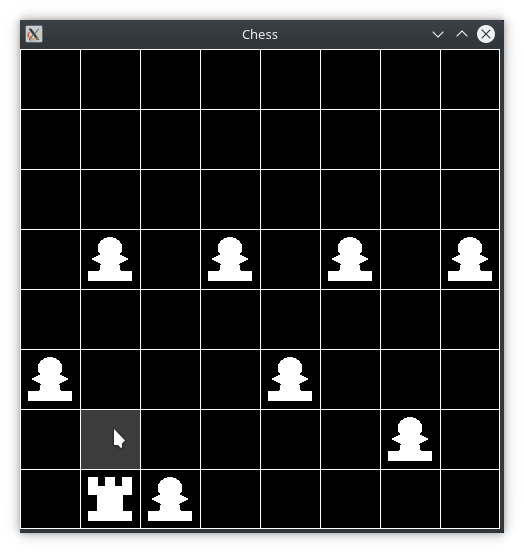
\includegraphics[width=\textwidth]{screenshot}
	\caption{Grafische Anwendung}
\end{figure}

\newpage
\section*{Quellcode}


\definecolor{deepblue}{rgb}{0,0,0.5}
\definecolor{deepred}{rgb}{0.6,0,0}
\definecolor{deepgreen}{rgb}{0,0.5,0}
\lstset{
	basicstyle=\ttfamily\footnotesize,
	language=C,
	tabsize=2,
	xleftmargin=-2.2cm,
	keywordstyle=\color{deepblue},
	emphstyle=\color{deepred},    % Custom highlighting style
	stringstyle=\color{deepgreen},
	frame=tb,                         % Any extra options here
	showstringspaces=false
}
\lstinputlisting[title=game.cpp]{../chessim/game.cpp}
\lstinputlisting[title=game.h]{../chessim/game.h}
\lstinputlisting[title=chess.cpp]{../chessim/chess.cpp}
\lstinputlisting[title=draw.cpp]{../chessim/draw.cpp}
\lstinputlisting[title=draw.h]{../chessim/draw.h}
\lstinputlisting[title=textInterface.h]{../chessim/textInterface.h}
\end{document}